\chapter{Conceptual model}

\section{Epidemiological model}
\label{concept_epidemiological_model}

The chosen epidemiological model to implement in the simulation contains six states: Susceptible, Symptomatic, Asymptomatic, Hospitalised, Recovered and Deceased (SIAHRD):
\begin{itemize}
    \item Susceptible (S) --- Agents in a Susceptible state are susceptible to infection by the virus. If in contact with an infected agent, they will in turn, with a probability, become infected and find themselves in the Symptomatic or Asymptomatic state.
    \item Symptomatic (I) --- Those in the Symptomatic state are contagious and can, after a period of time, either be put in the Hospitalised state, meaning their case has worsened, or end up in the Recovered state.
    \item Asymptomatic (A) --- In the Asymptomatic state, agents are contagious. But as they are lacking any signs of the disease, they are perceived by others as uninfected. After giving a quick and effective immune response against the virus, asymptomatic agents will directly go to the Recovered state.
    \item Hospitalised (H) --- Agents in the Hospitalised state are taken aside --- for treatment, as taken into a hospital --- and will infect no other agent. These hospitalised agents stay secluded for a certain time until they end up in either the Recovered state or the Deceased state.
    \item Recovered (R) --- The Recovered state is a state in which agents were previously infected by the virus and are now immune to it during some time. After the immune system has decreased in strength, recovered agents will again find themselves susceptible to infection in the Susceptible state.
    \item Deceased (D) --- The Deceased state is a final state. Agents fall in this state when they have succumbed to the disease.
\end{itemize}

The three basic classes of a compartmental model in epidemiology are S, I and R, as stated in section \ref{mathematical_models}. One cannot model an epidemic without them. The Asymptomatic state was chosen as vaccines give a higher chance to get asymptomatic once infected. This state will also play a significant role in conjunction with influence over trust (see section \ref{trust_agent_interactions} further on). As vaccines are intended to protect against harmful diseases, the Hospitalised state was added to represent infected agents highly suffering from their diseases (e.g., shortness of breath). If an agent does not recover from a Hospitalised state, then it has passed away, thus the existence of the Deceased state.

\begin{figure}
    \begin{minipage}{\textwidth}
        \centering
        \begin{tikzpicture}[->, >=stealth', shorten >=1pt, auto, node distance=2.8cm, semithick]
            \node[state] (S)              {$S$};
            \node[state] (I) [right of=S] {$I$};
            \node[state] (A) [below of=I] {$A$};
            \node[state] (H) [right of=I] {$H$};
            \node[state] (D) [right of=H] {$D$};
            \node[state] (R) [below of=D] {$R$};
            \path   (S) edge                node {$P(I)$} (I)
                        edge                node {$P(A)$} (A)
                    (I) edge                node {$P(H)$} (H)
                        edge                node {$P(Ri)$} (R)
                    (A) edge                node {$P(Ra)$} (R)
                    (H) edge                node {$P(Rh)$} (R)
                        edge                node {$P(D)$} (D)
                    (R) edge [bend left=80] node {$P(S)$} (S);
        \end{tikzpicture}
    \end{minipage}

    \begin{minipage}{\textwidth}
        \begin{align*}
            P(T) &= 1/4 \\
            P(I) &= 1 - P(A) \\
            P(A) &= P(T) + 1/8 \\
            P(H) &= 7/20&, \textnormal{with random duration } i \sim \mathcal{N}(2.1, 0.1) \\
            P(D) &= 1/4&, \textnormal{with random duration } h \sim \mathcal{N}(1.0, 0.3) \\
            P(Ri) &= 1 - P(H) \\
            P(Rh) &= 1 - P(D) \\
            P(Ra) &= 1&, \textnormal{with random duration } a \sim \mathcal{N}(1.5, 0.2) \\
            P(S) &= 1/4&, \textnormal{with random duration } r \sim \mathcal{N}(6, 3)
        \end{align*}
    \end{minipage}
    \caption{SIAHRD epidemiological model for unvaccinated agents followed by its state transition probabilities and random state visit duration.
    \label{fig:epidemiological_model}}
\end{figure}

An unvaccinated agent's epidemiological state will follow the probabilities part of the epidemiological model presented in figure \ref{fig:epidemiological_model}.
All constants as well as means and variances applied to the normal distribution of random state visit duration variables $i$, $h$, $a$ and $r$ are based on SARS-CoV-2's Delta variant for which all values are divided by 10 \cite{rozier_covidtracker_nodate, altarawneh_protection_2022, wong_high_2020, faes_time_2020}. The SARS-CoV-2's Delta variant was chosen because its values were the easiest to gather and retrieve. Additionally, as a reminder, the goal for this simulation is to educate and not to predict. These constants need not be exact, but at least approximated.

All four state visit duration variables $i$, $h$, $a$ and $r$ represent the number of days needed before a change of state. Again, the original values were divided by 10 to accelerate the process. In reality, an agent would stay 21 days with a variance of 1 ($i$) in the Symptomatic state before changing to the Hospitalised state. Once in the Hospitalised state, the agent would stay in it for 10 days with a variance of 3 ($h$). An agent would stay 15 days in the Asymptomatic state with a variance of 2 ($a$) before recovering. Finally, an agent would stay in the Recovered state 60 days with a variance of 30 ($r$) before becoming, once again, susceptible to infection.

The probability for the virus to be transmitted from an agent to another, defined as $P(T)$, is equal to one quarter. Once the virus is transmitted, the newly infected agent either changes its epidemiological state to the Symptomatic state or to the Asymptomatic state. $P(A)$ is the state transition probability for an agent to fall into the Asymptomatic state, which is equal to an eighth added to $P(T)$. If not in the Asymptomatic state, agents fall into the Symptomatic state, hence obtaining the state transition probability to be in the Symptomatic state $P(I)$ through the complement of $P(A)$. From a Symptomatic state, an agent can get to a Hospitalised state with a state transition probability $P(H)$ equal to seven-twentieths after a random duration $i$ following a normal distribution of mean 2.1 and of variance 0.1. Similarly, from a Hospitalised state, an agent can find itself in a Deceased state with a state transition probability $P(D)$ equal to one quarter after a random duration $h$ following a normal distribution of mean 1.0 and of variance 0.3. There are three ways for an agent's epidemiological state to become Recovered. The state transition probability $P(Ri)$ to get to a Recovered state from the Symptomatic state is the complement of $P(H)$. The state transition probability $P(Rh)$ to get to a Recovered state from the Hospitalised state is the complement of $P(D)$. And the state transition probability $P(Ra)$ to get to a Recovered state from the Asymptomatic state is equal to a random duration $a$ following a normal distribution of mean 1.5 and of variance 0.2. Finally, $P(S)$ is the state transition probability for an agent in the Recovered state to get back to a Susceptible state, which is equal to one quarter after a random duration following a normal distribution of mean 6 and of variance 3.

\section{Vaccination status}
\label{concept_vaccination_status}

Agents are given an additional attribute showing their vaccination status, which is different from a health state or an epidemiological state. Agents are either vaccinated, or they are not. The vaccination status attribute plays a role in the probability for agents to get infected, in the probability for agents to show symptoms, in the time it takes them to recover from their infection, and by influencing the chances they have to not get hospitalised, nor die. In other words, a good vaccine makes vaccinated agents have fewer chances to get infected by other agents and higher chances to be asymptomatic if infected. It will also enable faster recovery from an infected state and prevent vaccinated agents from getting hospitalised. Basically, the vaccination status attribute influences the probability to get from one state of the epidemiological model to another.

Only agents in the Susceptible and Asymptomatic states can get vaccinated. Asymptomatic agents do not show any symptoms and, without screening, they cannot tell if they caught the virus or not. Agents with a Symptomatic or Hospitalised epidemiological state, following institutions' and medical organisations' guidelines and recommendations \cite{who_vaccine_advice_2022}, will not get vaccinated. And when in the Recovered state, agents are already immune to the disease by previously catching the virus. As for the Deceased state, agents are considered dead. Vaccination is thus useless for agents in the Deceased state.

Among all agents in a Susceptible and Asymptomatic state, only those "willing" to get vaccinated --- through probability entirely based on their trust level --- will get vaccinated.

A vaccinated agent will stay vaccinated for a limited duration. Once the limit reached, agents will lose their vaccination status. Being now unvaccinated, agents' epidemiological state will change following the compartment model without vaccination (see figure  \ref{fig:epidemiological_model}). They may, however, vaccinate themselves again.

\begin{figure}
    \begin{minipage}{\textwidth}
        \centering
        \begin{tikzpicture}[->, >=stealth', shorten >=1pt, auto, node distance=2.8cm, semithick]
            \node[state] (S)              {$S$};
            \node[state] (I) [right of=S] {$I$};
            \node[state] (A) [below of=I] {$A$};
            \node[state] (H) [right of=I] {$H$};
            \node[state] (D) [right of=H] {$D$};
            \node[state] (R) [below of=D] {$R$};
            \path   (S) edge                node {} (I)
                        edge                node {} (A)
                    (I) edge                node {} (H)
                        edge                node {} (R)
                    (A) edge                node {} (R)
                    (H) edge                node {} (R)
                        edge                node {} (D)
                    (R) edge [bend left=80] node {} (S)
                    
                    (S) edge [dashed, bend left=10] node {$P(Iv)$} (I)
                        edge [dashed, bend left=10] node {$P(Av)$} (A)
                    (I) edge [dashed, bend left=10] node {$P(Hv)$} (H)
                        edge [dashed, bend left=10] node {$P(Riv)$} (R)
                    (A) edge [dashed, bend left=10] node {$P(Rav)$} (R)
                    (H) edge [dashed, bend left=10] node {$P(Rhv)$} (R)
                        edge [dashed, bend left=10] node {$P(Dv)$} (D)
                    (R) edge [dashed, bend left=90] node {$P(Sv)$} (S);
            \matrix [draw, above left] at (current bounding box.south) {
                \node at (100pt, -3pt) [label=right:{unvaccinated}] {};
                \draw (60pt, 0pt) -- (100pt, 0pt); \\
                \node at (100pt, -3pt) [label=right:{vaccinated}] {};
                \draw [dashed] (60pt, 0pt) -- (100pt, 0pt); \\
            };
        \end{tikzpicture}
    \end{minipage}

    \begin{minipage}{\textwidth}
        \begin{align*}
            P(Tv) &= P(T) * (1 - 0.9) \\
            P(Iv) &= 1 - P(Av) \\
            P(Av) &= P(A) * 0.9 \\
            P(Hv) &= P(H) * (1 - 0.9)&, \textnormal{with random duration } i \sim \mathcal{N}(2.1, 0.1) \\
            P(Dv) &= P(D) * (1 - 0.9)&, \textnormal{with random duration } h \sim \mathcal{N}(1.0, 0.3) \\
            P(Riv) &= P(Ri) \\
            P(Rhv) &= P(Rh) \\
            P(Rav) &= P(Ra)&, \textnormal{with random duration } a \sim \mathcal{N}(1.5, 0.2) \\
            P(Sv) &= P(S) * (1 - 0.9)&, \textnormal{with random duration } r \sim \mathcal{N}(6, 3)
        \end{align*}
    \end{minipage}
    \caption{SIAHRD epidemiological model for vaccinated agents followed by its state transition probabilities and random state visit duration.
    \label{fig:epidemiological_model_vaccination}}
\end{figure}

A vaccinated agent's epidemiological state will follow the probabilities from the epidemiological model presented in figure \ref{fig:epidemiological_model_vaccination}.
As the vaccine's effectiveness acts as an inhibitor on probabilities without vaccination and that COVID-19 vaccines are not one hundred percent effective, it has been chosen to fix the vaccine's effectiveness to a float constant of 0.9 for 90\% overall effectiveness.

The state transition probability $P(Tv)$ for the virus to be transmitted from a contaminated agent, without giving importance to its vaccination status, to a vaccinated agent is equal to the probability $P(T)$ for the virus to be transmitted to any agent multiplied by the complement of the vaccine's effectiveness. As an example, if the vaccine is extremely effective and has a value of 1.0, the probability $P(T)$ would be nullified and no transmission of the virus would take place. Once again, after the transmission of the virus, the epidemiological state of a newly infected and vaccinated agent becomes either Symptomatic or Asymptomatic. The state transition probability $P(Av)$ for the epidemiological state of a vaccinated agent to be Asymptomatic is equal to the probability $P(A)$ for the epidemiological state of any agent to be Asymptomatic times the effectiveness of the vaccine. If not Asymptomatic, the state falls into the Symptomatic state, for which the state transition probability $P(Iv)$ is the complement of $P(Av)$. The state transition probability $P(Hv)$ for the Symptomatic epidemiological state of an agent to become Hospitalised is equal to $P(H)$ to which is multiplied the complement of the vaccine's effectiveness, just as the state transition probability $P(Dv)$ for an agent with a Hospitalised state to fall dead is $P(D)$ times the complement of the vaccine's effectiveness and that the state transition probability $P(Sv)$ for an agent with a Recovered state to become Susceptible again is $P(S)$ times the complement of the vaccine's effectiveness. Finally, the state transition probabilities for the epidemiological state of a vaccinated agent to become Recovered either from a Symptomatic state $P(Riv)$, a Hospitalised state $P(Rhv)$ or an Asymptomatic state $P(Rav)$ are the same as the ones with an unvaccinated agent.

\section{Trust and agent interactions}
\label{trust_agent_interactions}

Agents possess a trust level attribute represented by a real number normalised between 0.0 and 1.0. Ideally, this attribute would be initialised for all agents following a skew normal distribution, aiming at getting as close to an average trust level given by the user to the entire population of the simulation.
An agent expresses trust if its trust level is greater than 0.5 and expresses distrust if its trust level is less than 0.5.
This trust level attribute influences the agent's decision to vaccinate itself. An agent with a high trust level will be more likely to get vaccinated than an agent with a low trust level. Simply put, the probability for an agent to get vaccinated is its trust level. An agent's trust level can get updated through three different means:
\begin{enumerate}
    \item Interpersonal influence --- Agents in contact with each other will influence themselves into adjusting their trust level towards the one of the approached agent (figure \ref{fig:interpersonal_influence}). This adjustment depends on the degree of polarisation of their trust level. A highly polarised agent will be highly influential and barely influenced by others, while an agent with a moderately or slightly polarised trust level will be less influential and more susceptible to being influenced by others.

    \item Observational influence --- Agents inform themselves about the symptomatic and vaccination states of other agents in their surroundings, as well as themselves (figure \ref{fig:observational_influence}). Depending on whether neighbouring agents are vaccinated and/or symptomatic (Symptomatic or Hospitalised state), the observing agent's trust level will get updated. Observed agents that are vaccinated and showing symptoms will decrease the trust of the observing agent, while observed agents that are vaccinated and that do not show any symptoms will increase the trust of the observing agent. This makes the asymptomatic state a crucial element to add to this simulation, as an agent surrounded by vaccinated agents in a Asymptomatic state will think that the vaccine is efficient. Additionally, randomly selected agents will visit agents with a Hospitalised epidemiological state which were put aside in order to update those selected agents' trust level by this means of influence.

    \item Institutional influence --- Similar to the observational influence, agents receive global information about the current situation among hospitalised and deceased agents (figure \ref{fig:institutional_influence}). For both epidemic states, separately, the information informs about the proportion of vaccinated agents in one of these epidemic states against the proportion of vaccinated agents not in the epidemic state of concern. If the information shows that 10\% of hospitalised agents are vaccinated and that 90\% of the rest of the population is vaccinated, then the vaccine will seem effective. But if the information shows that 50\% of hospitalised agents are vaccinated and that 50\% of the rest of the population is vaccinated, then the vaccine will seem useless. Additionally, this global information will be wrongly interpreted by half of the population to show the difference in the outcome of the epidemic between a correctly interpreting population and a wrongly interpreting population. This misinterpreting half of the population will only assimilate the proportion of vaccinated agents in the epidemiological states of concern (Hospitalised and Deceased) without keeping track of the proportion of vaccinated in the rest of the population. In other words, agents may show difficulties in completely understanding the statistics given to them \cite{francetvinfo_morts_vaccines_2021, lesoir_infographie_hospitalises_vaccines_2021}. For example, if agents perceive the information that 90\% of hospitalised agents are vaccinated regardless of the proportion of vaccinated agents in the rest of the population, they might think that the vaccine is useless or counter-effective.
\end{enumerate}

\begin{figure}[!htb]
    \centering
    \minipage{0.38\textwidth}
        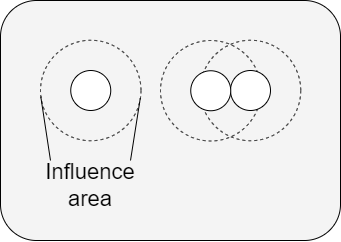
\includegraphics[width=\linewidth]{pics/interpersonal.drawio.png}
    \endminipage
    \caption{Interpersonal influence - Agents close enough to each other will influence each other's trust. On the right, two agents are close enough to update their trust levels between themselves.}
    \label{fig:interpersonal_influence}
\end{figure}
\begin{figure}[!htb]
    \centering
    \minipage{0.48\textwidth}
        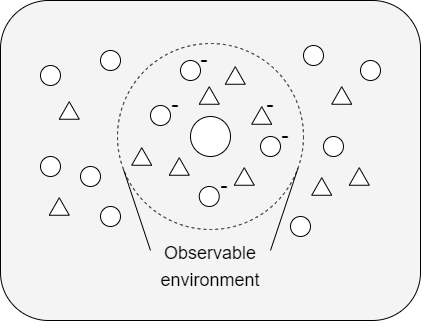
\includegraphics[width=\linewidth]{pics/observational.drawio.png}
    \endminipage
    \caption{Observational influence - Agents will observe their environment and update their own trust level based on their observations. The observing agent (big circle) can see four unvaccinated agents (small circles) with symptoms (\babelhyphen{nobreak}), five vaccinated agents (small triangles) without symptoms and one vaccinated agent with symptoms.}
    \label{fig:observational_influence}
\end{figure}

\clearpage

\begin{figure}[!htb]
    \centering
    \minipage{0.58\textwidth}
        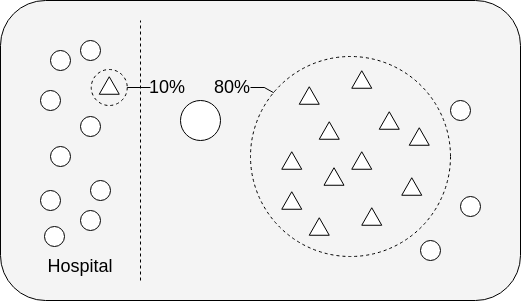
\includegraphics[width=\linewidth]{pics/institutional.drawio.png}
    \endminipage
    \caption{Institutional influence - Agents will receive information about the proportion of vaccinated agents in and out of a specific epidemiological state. The aware agent (big circle) is informed that 10\% of hospitalised agents are vaccinated and that 80\% of unhospitalised agents are vaccinated.}
    \label{fig:institutional_influence}
\end{figure}

\begin{figure}[!htb]
    \centering
    \minipage{0.34\textwidth}
        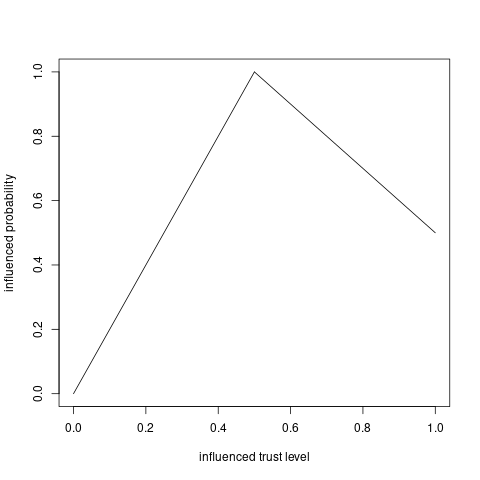
\includegraphics[width=\linewidth]{pics/influenced_probability.png}
        \caption{Probability to be influenced based on the influenced agent's trust level}
        \label{fig:influenced_probability}
    \endminipage
    \hspace{0.2in}
    \minipage{0.34\textwidth}
        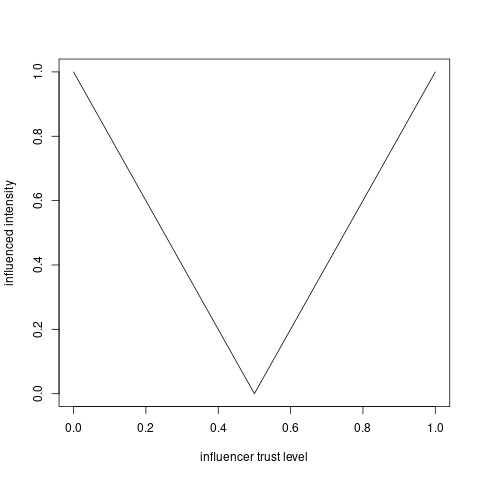
\includegraphics[width=\linewidth]{pics/influence_intensity.png}
        \caption{Intensity of the influence based on the influencer agent's trust level}
        \label{fig:influence_intensity}
    \endminipage
    \\
    \minipage{\textwidth}
        \centering
        \minipage{0.34\textwidth}
            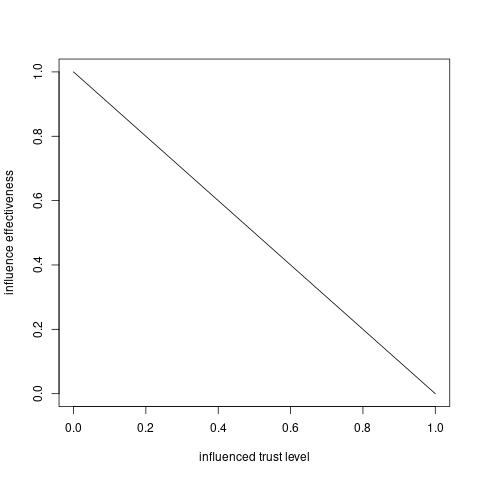
\includegraphics[width=\linewidth]{pics/influence_effectiveness_below.png}
        \endminipage
        \hspace{0.2in}
        \minipage{0.34\textwidth}
            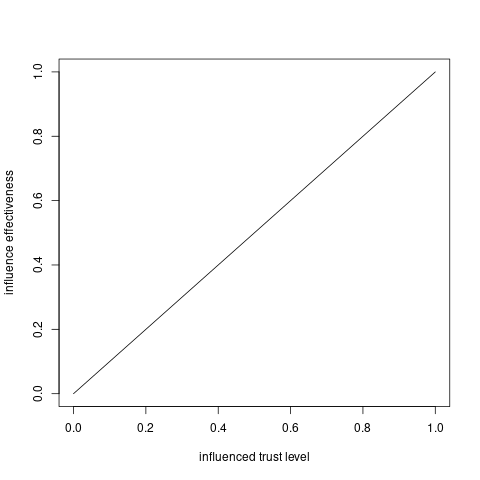
\includegraphics[width=\linewidth]{pics/influence_effectiveness_above.png}
        \endminipage
        \captionsetup{width=0.82\linewidth}
        \caption{Effectiveness of the influence based on the influenced agent's trust level whether the influencer agent's trust level is below 0.5 (left) or above 0.5 (right)}
        \label{fig:influence_effectiveness}
    \endminipage
\end{figure}

\pagebreak

\subsection{Interpersonal influence over trust}
When an agent comes into close contact with another agent upon entering a predefined influence area (figure \ref{fig:interpersonal_influence}) --- these areas surround each agent ---, it will be influenced by the other agent's trust level with a probability based on its own trust level. The other agent will obviously, in turn, be influenced by the first agent's trust level with a probability calculated similarly. See algorithm \ref{algo:interpersonal}.

Distrusting agents possess a trust level below 0.5. The probability $P(DI)$ for a distrusting agent to be influenced based on its trust level $tl$ is:
\[P(DI) = tl / 0.5\]

Trusting agents have a trust level above 0.5. The probability $P(TI)$ for a trusting agent to be influenced based on its trust level $tl$ is:
\[P(TI) = 0.5 + (1 - tl)\]

These two probabilities are represented in figure \ref{fig:influenced_probability} in which it is possible to see that in order to make distrusting agents (in range [0.0, 0.5[) less influenced than trusting agents (in range ]0.5, 1.0]), $P(DI)$ creates a linear probability distribution ranging from 0.0 to 1.0, while $P(TI)$ results in a linear probability distribution ranging from 0.5 to 1.0. This makes trusting agents susceptible to being influenced at least half of the time. If the probability is in favour of the influencer, a calculation is run to determine how much the trust level of the influenced agent is to be updated.

In order to determine the update to apply to the influenced agent's trust level, the intensity and the effectiveness of the influence need to be calculated. The intensity of the influence is based on the influencer's trust level and ranges piece-wise linearly from 0 to 1 for a trust level ranging from 0 to 0.5 and ranging from 0.5 to 1 (figure \ref{fig:influence_intensity}). The effectiveness of the influence is based on both the influencer agent's and the influenced agent's trust levels. If the influencer's trust level is below 0.5, then the influence effectiveness ranges linearly from 0 to 1 for an influenced trust level ranging from 1 to 0. If the influencer's trust level is above 0.5, then the influence effectiveness ranges linearly from 0 to 1 for an influenced trust level ranging from 0 to 1 (figure \ref{fig:influence_effectiveness}).

Once the intensity and the effectiveness calculated, the update to apply to the influenced agent's trust level is the multiplication of both, times -1 if the influencer agent's trust level is below 0.5.

\pagebreak

\begin{algorithm}[language=Pseudocode, caption={Interpersonal influence over trust}, label={pseudo_code_interpersonal}]
agents: list of all agents
get_alive_agents_in_contact(X): get all agents not deceased in agent X's surroundings within a fixed NetLogo radius of 0.1
random(f): produce a uniform distribution
begin
    for each influencer in agents do
        if not (influencer.is_hospitalised or influencer.is_deceased) then
            agents_in_contact <- get_alive_agents_in_contact(influencer)
            for each influenced in agents_in_contact do
                if influenced.trust_level < 0.5 then
                    probability_influenced <- random(influenced.trust_level / 0.5)
                else
                    probability_influenced <- random(0.5 + (1 - influenced.trust_level))
                end if
                if probability_influenced > random(1) then
                    if influencer.trust_level < 0.5 then
                        influence_intensity <- 1 - (influencer_trust_level / 0.5)
                        influence_effectiveness <- 1 - trust-level
                        influence_update <- influence_intensity * influence_effectiveness
                        influenced_trust_level <- influenced_trust_level - influence_update
                    else if influencer.trust_level > 0.5 then
                        influence_intensity <- (influencer_trust_level / 0.5) - 1
                        influence_effectiveness <- trust-level
                        influence_update <- influence_intensity * influence_effectiveness
                        influenced_trust_level <- influenced_trust_level + influence_update
                    else
                        influenced_trust_level <- influenced_trust_level
                    end if
                end if
            end for
        end if
    end for
end
\end{algorithm}

\begin{algorithm}[language=Pseudocode, caption={Observational influence over trust}, label={pseudo_code_observational}]
agents: list of all agents
get_alive_agents_in_surroundings(X): get all agents not deceased in agent X's surroundings within a fixed NetLogo radius of 0.5
begin
    for each observer in agents do
        if not (observer.is_hospitalised or observer.is_deceased) then
            agents_in_surroundings <- get_alive_agents_in_surroundings(observer)
            for each other in agents_in_surroundings do
                if other.is_vaccinated and not other.is_symptomatic then
                    observer.trust_level <- observer.trust_level + (0.03 * observer.trust_level)
                else if other.is_vaccinated and other.is_symptomatic then
                    observer.trust_level <- observer.trust_level - (0.05 * (1 - observer.trust_level))
                end if
            end for
        end if
    end for
end
\end{algorithm}

\subsection{Observational influence over trust}

Agents in a physical state that allows them to observe their environment will update their trust level based on their observation of vaccinated agents. Those observing agents are all agents, with exception to those having a Hospitalised or a Deceased epidemic state. There are two possible cases. If the observer agent sees a vaccinated and asymptomatic agent (other than in the Symptomatic or Hospitalised epidemic state), which is positive information, then its trust level will slightly increase. However, if the observer agent sees a vaccinated and symptomatic agent (in the Symptomatic or Hospitalised epidemic state), negative information, then its trust level will decrease more than in would have increased \cite{cvetkovich_new_2002}. These increases and decreases are small percentages (3\% and 5\%) of the observer agent's own trust level, working as a confirmation bias \cite{nickerson_confirmation_1998}. In addition, trusting agents will tend to ignore negative information as distrusting agents will tend to neglect positive information \cite{cvetkovich_new_2002}. See algorithm \ref{algo:observational}.

\subsection{Institutional influence over trust}
\label{conception_institutional}

Agents other than in a Hospitalised or Deceased epidemiological state will get their trust level updated according to the received information and their own trust level. In order to update all attentive agents' trust level, (a) the proportion of vaccinated agents among the epidemiological state of concern and (b) the proportion of all other alive vaccinated agents in the environment must first be calculated. The difference between those two proportions (b - a) --- divided by 1000 to lighten its effect --- is then used to create the value by which to update. If the difference is above 0, the type of the information is considered positive. If the difference is below 0, the type of the information is considered negative. The difference is then attenuated and adjusted with each agent's trust level depending on the information type (confirmation bias \cite{nickerson_confirmation_1998}) before finally becoming the update value to apply independently to each agent. Additionally, the option to make that information incomplete was added. See algorithm \ref{algo:institutional}.

\begin{algorithm}[language=Pseudocode, caption={Institutional influence over trust}, label={pseudo_code_institutional}]
agents: list of all agents
proportion_X_vaccinated: percentage of vaccinated among agents with an epidemiological state X
proportion_not_X_vaccinated: percentage of vaccinated not among agents with an epidemiological state X
begin
    for each agent in agents do
        if not (agent.is_hospitalised or agent.is_deceased) then
            if agent.misinterprets then
                trust_level_update <- (proportion_X_vaccinated / 100) * -1 * (1 - agent.trust_level)
            else
                proportion_difference <- (proportion_not_X_vaccinated - proportion_X_vaccinated) / 100
                if proportion_difference >= 0 then
                    trust_level_update <- proportion_difference * 0.5 * agent.trust_level
                else
                    trust_level_update <- proportion_difference * (1 - agent.trust_level)
                end if
            end if
            agent.trust_level <- agent.trust_level + trust_level_update
        end if
    end for
end
\end{algorithm}
